\noindent{As candidates for events, these possible actions on classes are considered:}
\begin{itemize}
\item Submitting/Canceling votes:
    When a costumer votes for a track, or cancels it. If the \textbf{vote} fits within the \textbf{restrictions}, the voted for \textbf{track}s vote count is changed and potentially its order in the \textbf{playlist} class, the specific \textbf{costumer} vote is changed.
\item Checking in/out of venues:
    Costumer checks in at the venue, one wants to vote at. This allows the costumer to \textbf{vote}.
\item Searching for a track:
    When a costumer is searching for a desired track in the repertoire/catalogue of tracks. The costumer should recieve relevant search results that fit within the \textbf{restriction}s.
\item Adding/Removing a new track to the playlist:
    If the track a costumer voted for is not on the playlist already, or if the track only had one vote that got cancelled.
\item New track is playing:
    When a another track instance ended, due to being skipped or reached the end. This should affect the \textbf{vote} count of a \textbf{track}. If a \textbf{customer}s track is played his vote should be neglected.
\item Adding/Removing restrictions:
    When the administrator either adds or removes a restriction for the system, this may also be by time intervals. Already added \textbf{track} that does not meet the requirements should be neglected. Cascading through the specific \textbf{costumers} \textbf{vote}, and the \textbf{playlist}.
\end{itemize}

The following event table is used to describe what classes are involved in the immediate events of the problem domain:

\begin{center}
    \begin{tabular}{|l|l|l|l|l|l|}
    \hline
    \textbf{Events} & Costumer & Track & Playlist & Vote & Restriction \\ \hline
    (RE)vote & * & * & * & * &   \\ \hline
    Costumer checks in at venue & * &   &   & * &   \\ \hline
    Costumer leaves venue & * &   &   &   &   \\ \hline
    Costumer is searching for a track & * &   &   &  & * \\ \hline
    Adding a new track to the playlist & * & * & * & * &   \\ \hline
    Remove track from the playlist & * & * & * & * &   \\ \hline
    A new track is playing & * & * & * & * &   \\ \hline
    Restriction added & * & * & * & * & * \\ \hline
    Restriction removed & * & * & * & * & * \\ \hline
    \end{tabular}
\end{center}


\begin{figure}
  \centering
  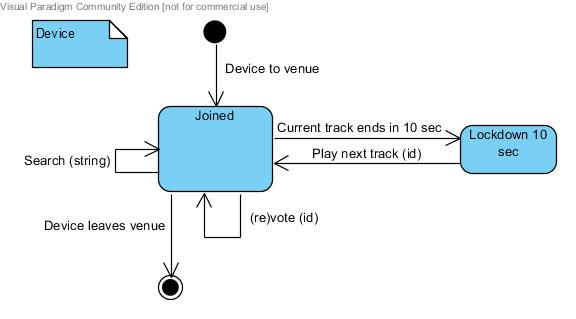
\includegraphics[width=\textwidth]{StateDiagramDevice.jpg}
  \caption{Class diagram of problem domain}\label{fig:StateDiagramDevice}
\end{figure}

\begin{figure}
  \centering
  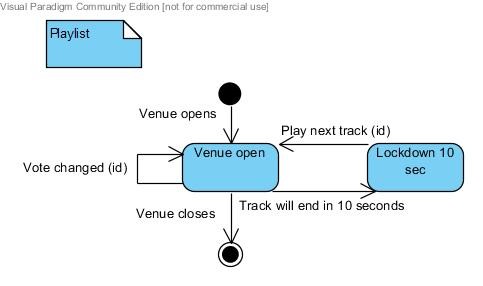
\includegraphics[width=\textwidth]{StateDiagramPlaylist.jpg}
  \caption{Class diagram of problem domain}\label{fig:StateDiagramPlaylist}
\end{figure}

\begin{figure}
  \centering
  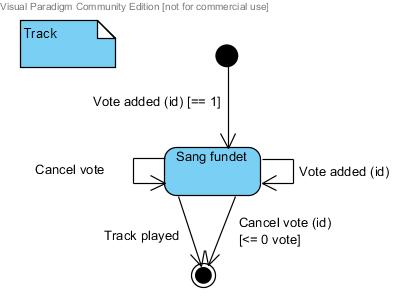
\includegraphics[width=\textwidth]{StateDiagramTrack.jpg}
  \caption{Class diagram of problem domain}\label{fig:StateDiagramTrack}
\end{figure}